\section{How to display everything?}

Right after the ``neighborlist'' object has been created, we can render the whole thing.
    \begin{figure}[h]
    \begin{centering}
    \caption{THe instance method ``render'' of the controller object}
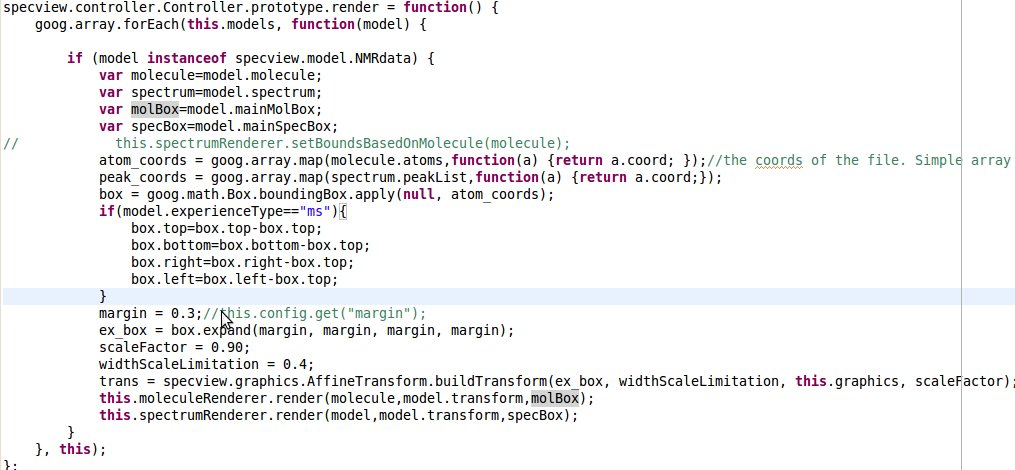
\includegraphics[width=200mm,height=95mm]{./images/renderController}
%    \label{subd}
    \end{centering}
    \end{figure}

At the end of this method are called             this.\textbf{moleculeRenderer}.render(molecule,model.transform,molBox) and 
            this.\textbf{spectrumRenderer}.render(model,model.transform,specBox).
``molceuleRenderer'' and ``spectrumRenderer'' are attributes of the controller object. More precisely they are classes  to render molecule and spectrum objects on graphics objects. These classes contain a instance method named ``render'' which properly draw the molecule(respectibely spectrum) object on the graphics object.
\clearpage

\textbf{Example of a renderer class}

    \begin{figure}[h]
    \begin{centering}
    \caption{The instance method render of the class spectrumRenderer}
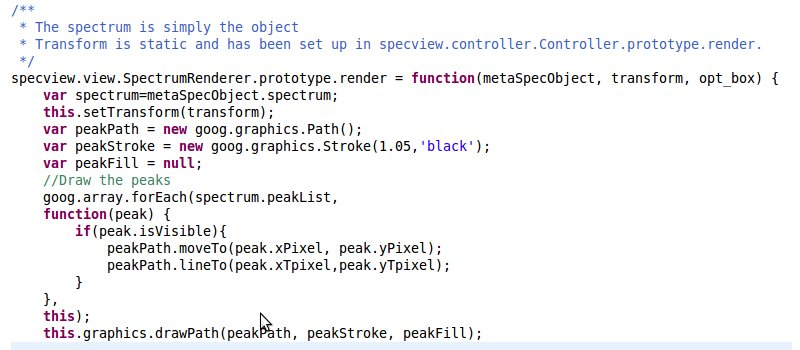
\includegraphics[width=190mm,height=75mm]{./images/spectrumRenderer}
%    \label{subd}
    \end{centering}
    \end{figure}

At each ``\textbf{this.graphics.drawPath(peakPath, peakStroke, peakFill)}'' a new peak is drawn on the canvas editor. 
\clearpage
